\section{Generation Details of Signal Sample}
\label{sec:MCsampleGeneration}
\subsection{Madgraph setup and parameters}

\begin{sloppypar}
Madgraph cards are located here: \url{https://github.com/cms-sw/genproductions/tree/pre2017/bin/MadGraph5_aMCatNLO/cards/production/13TeV/VBS/VVjj_semileptonic}
\end{sloppypar}

The gridpacks for signal can be found here:

\begin{sloppypar}
\url{/cvmfs/cms.cern.ch/phys\_generator/gridpacks/slc6\_amd64\_gcc481/13TeV/madgraph/V5\_2.4.2/AnomalousCouplingsSMP}
\end{sloppypar}

\subsection{How samples are generated?}
We generated our signal using Madgraph version V5\_2.4.2. The main setting used different from default run card are 
\begin{itemize}
	\item maxjetflavor = 5
	\item mjj = 100
\end{itemize}

\subsubsection{SM signal sample generation}
Signal sample was generated with pure electroweak vertex with option "QED=4 and QCD=0". Below you can see the proc card information. 

\begin{verbatim}
set group_subprocesses Auto
set ignore_six_quark_processes False
set loop_optimized_output True
set complex_mass_scheme False
import model sm-ckm_no_b_mass
define p = g u c d s b u~ c~ d~ s~ b~
define j = p 
define l+ = e+ mu+ ta+
define l- = e- mu- ta-
define vl = ve vm vt
define vl~ = ve~ vm~ vt~
generate p p > w+ w- j j QED=4 QCD=0 
output WPlepWMhadJJ_EWK_LO_SM_mjj100_pTj10 --nojpeg
\end{verbatim}

\subsubsection{aQGC signal sample generation}
aQGC sample generated with effective field theory with dimension eight effective operators assuming that the recently observed Higgs boson belongs to a SU(2)$_{L}$ doublet, with the method proposed by Eboli~\cite{Belyaev:1998ih,Eboli:2006wa,Eboli:2000ad,Eboli:2003nq}
\begin{verbatim}
set group_subprocesses Auto
set ignore_six_quark_processes False
set complex_mass_scheme False
import model SM_LS_LM_LT_UFO
define p = g u c d s u~ c~ d~ s~ 
define j = g u c d s u~ c~ d~ s~ b b~
define l+ = e+ mu+ ta+
define l- = e- mu- ta-
define vl = ve vm vt
define vl~ = ve~ vm~ vt~
generate p p > w- w+ j j QED=4 QCD=0 NP=1
output aQGC_WMhadWPlepJJ_EWK_LO_NPle1_mjj100pt10 --nojpeg
\end{verbatim}
To generate aQGC sample we used option {\bf NP=1}. This option forces madgraph to generate sample having SM, aQGC, and interference diagrams.
Also, we can not decay w-boson here with madgraph because of the limitation of the Madgraph. The issue is that madgraph uses only final state in order to identify which matrix-element to use but it can not able to distinguish which of the jets are coming from the $W^+$. This is the source of error. Here, you can follow the discussion with authors:
\begin{sloppypar}
	\url{https://bugs.launchpad.net/mg5amcnlo/+bug/1633803}
\end{sloppypar}
Used model can be found at generator repository of models: 
\begin{sloppypar}
https://cms-project-generators.web.cern.ch/cms-project-generators/ 
\end{sloppypar}

\subsection{Comparison of SM and aQGC distribution}

\begin{figure}[htb]
  \begin{center}
    \begin{tabular}{c}
    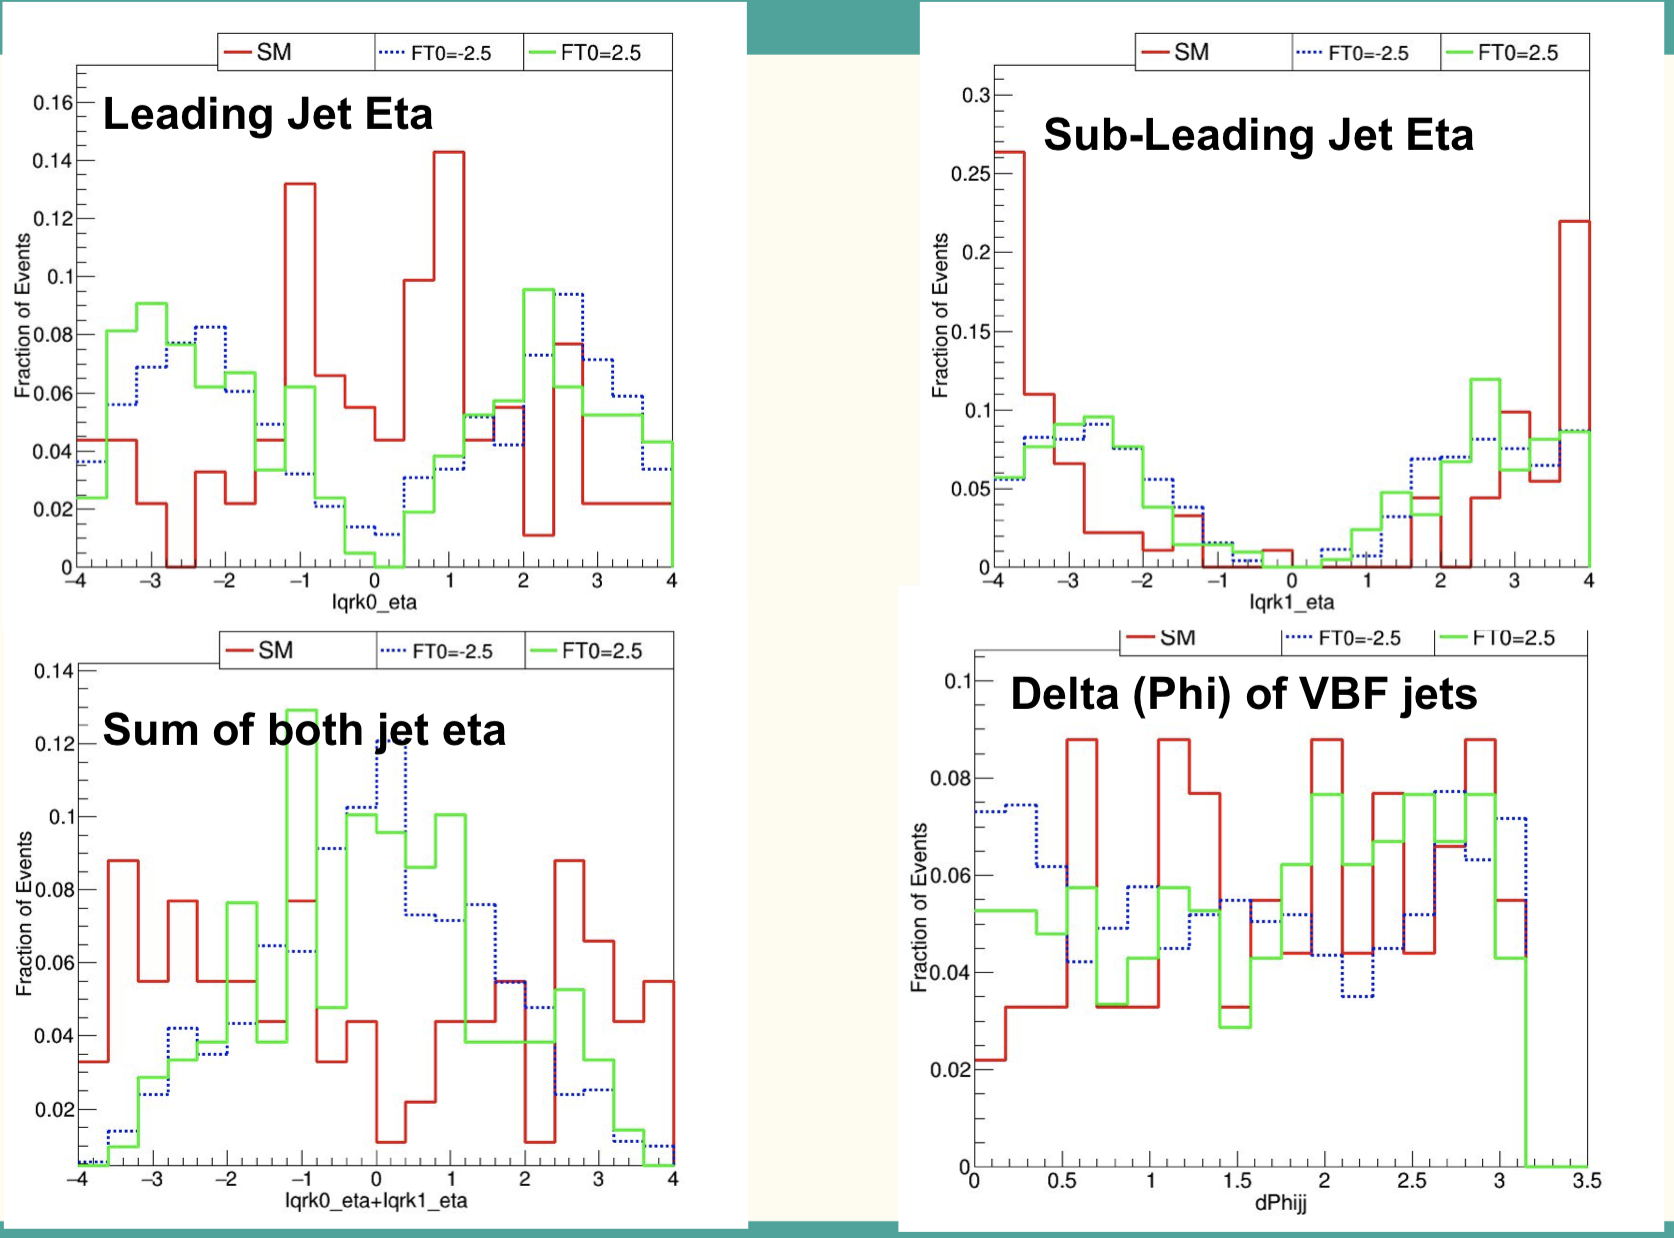
\includegraphics[width=1.00\textwidth]{Plots/GenLevelStudy/pic1.png}    \end{tabular}
    \caption{VBF jets distribution}
    \label{fig:gen1}
  \end{center}
\end{figure}
\begin{figure}[htb]
  \begin{center}
    \begin{tabular}{c}
    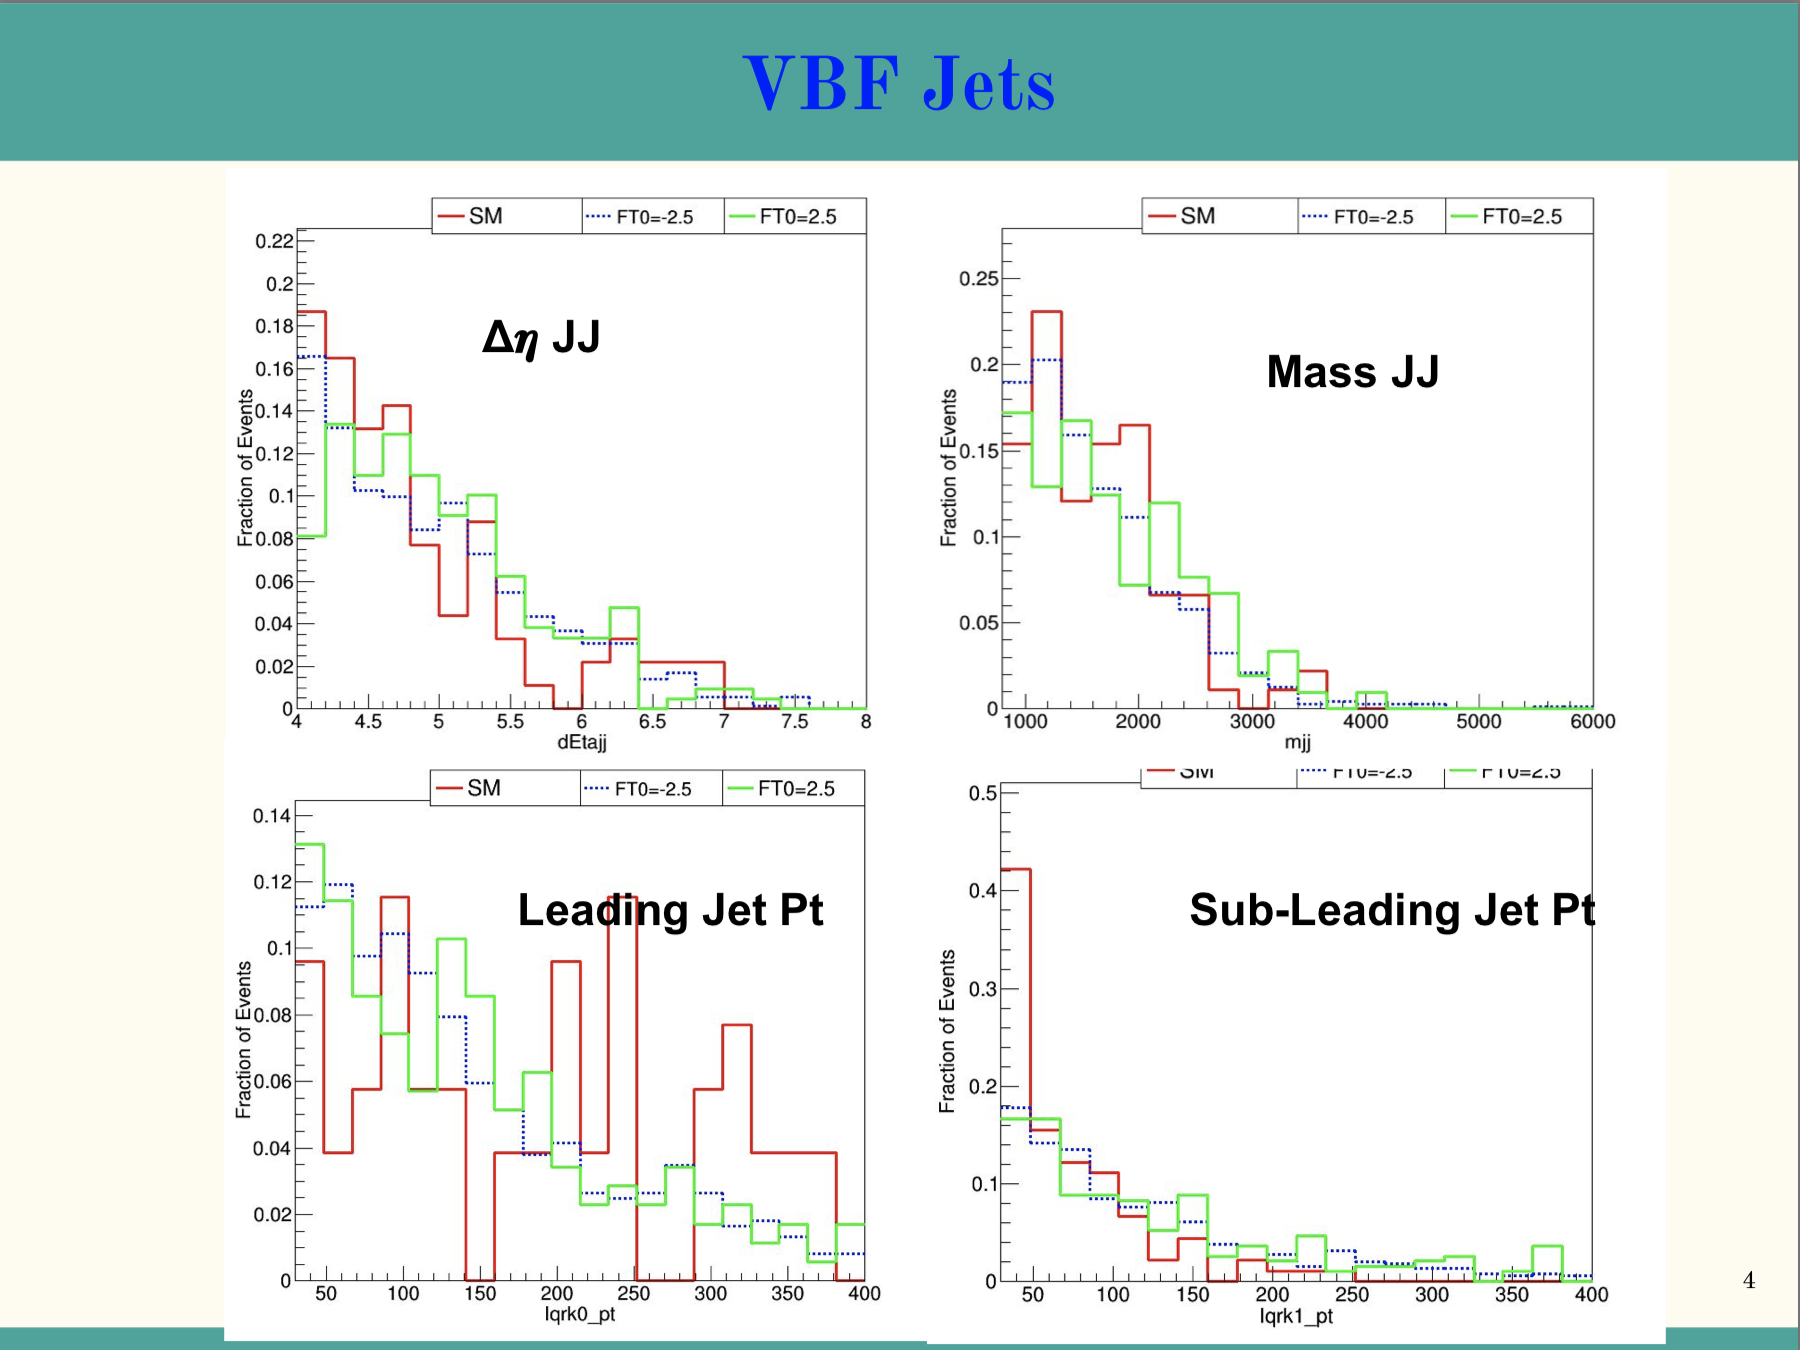
\includegraphics[width=1.00\textwidth]{Plots/GenLevelStudy/pic3.png}\\
    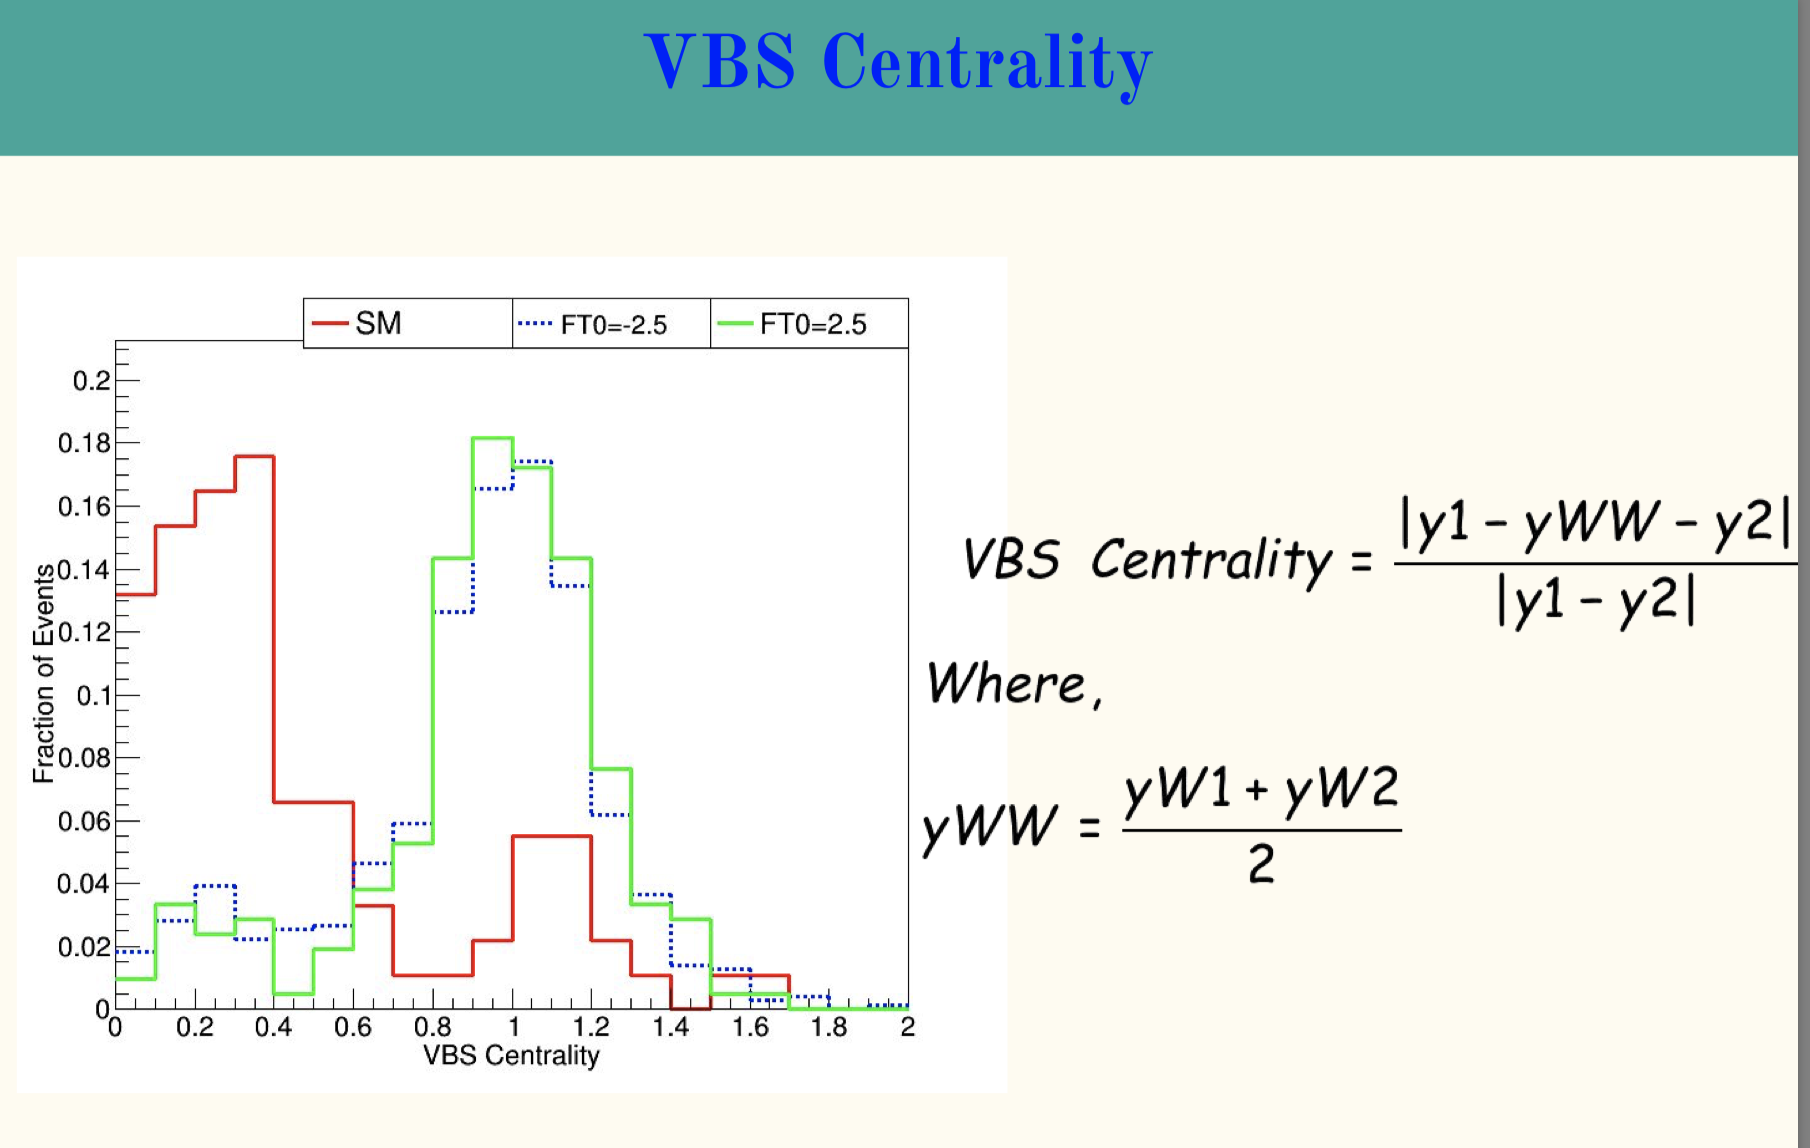
\includegraphics[width=1.00\textwidth]{Plots/GenLevelStudy/pic4.png}    \end{tabular}
    \caption{Top: VBF jets distribution. Bottom: VBS centrality}
    \label{fig:gen2}
  \end{center}
\end{figure}
\begin{figure}[htb]
  \begin{center}
    \begin{tabular}{c}
    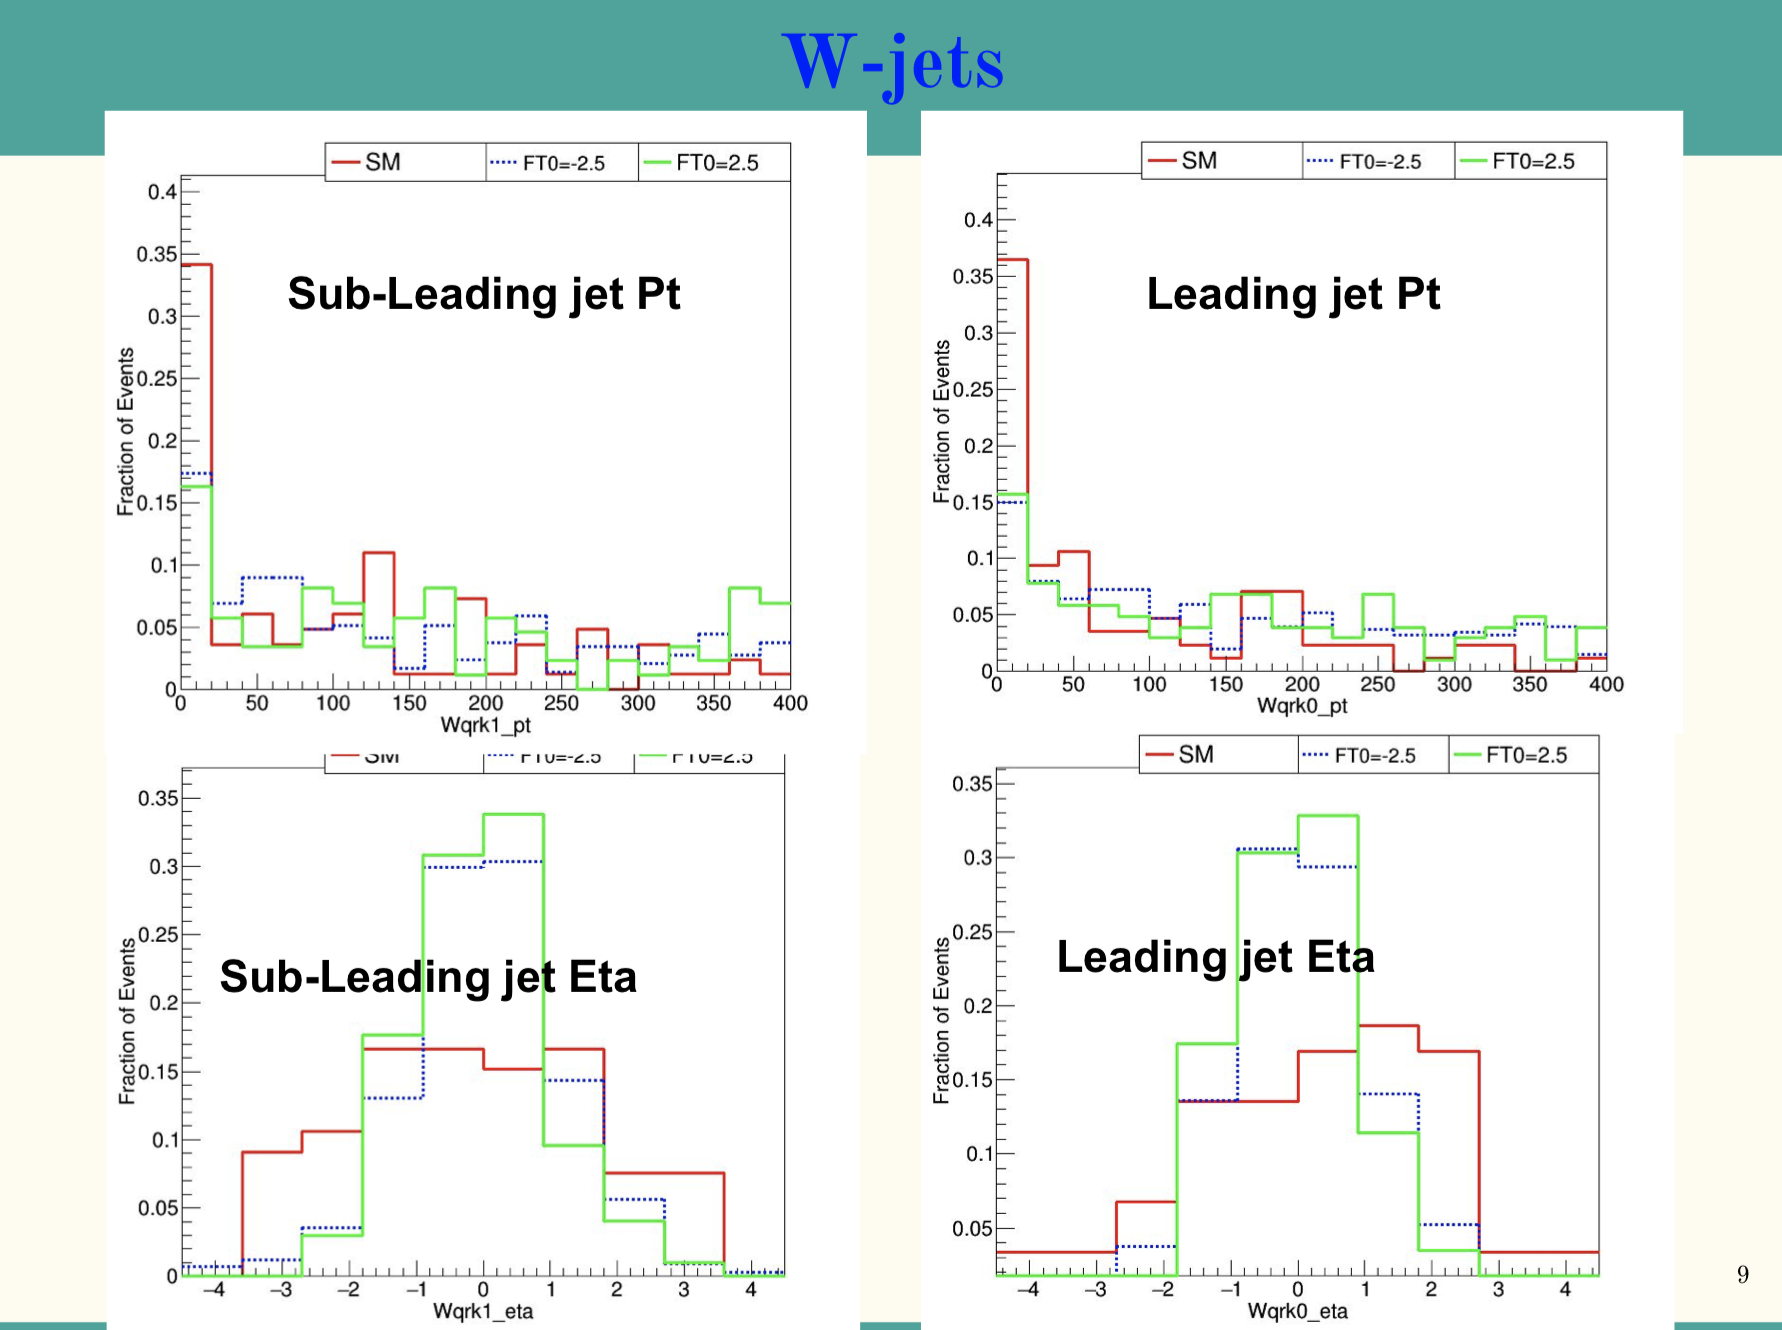
\includegraphics[width=0.90\textwidth]{Plots/GenLevelStudy/pic5.png}\\
    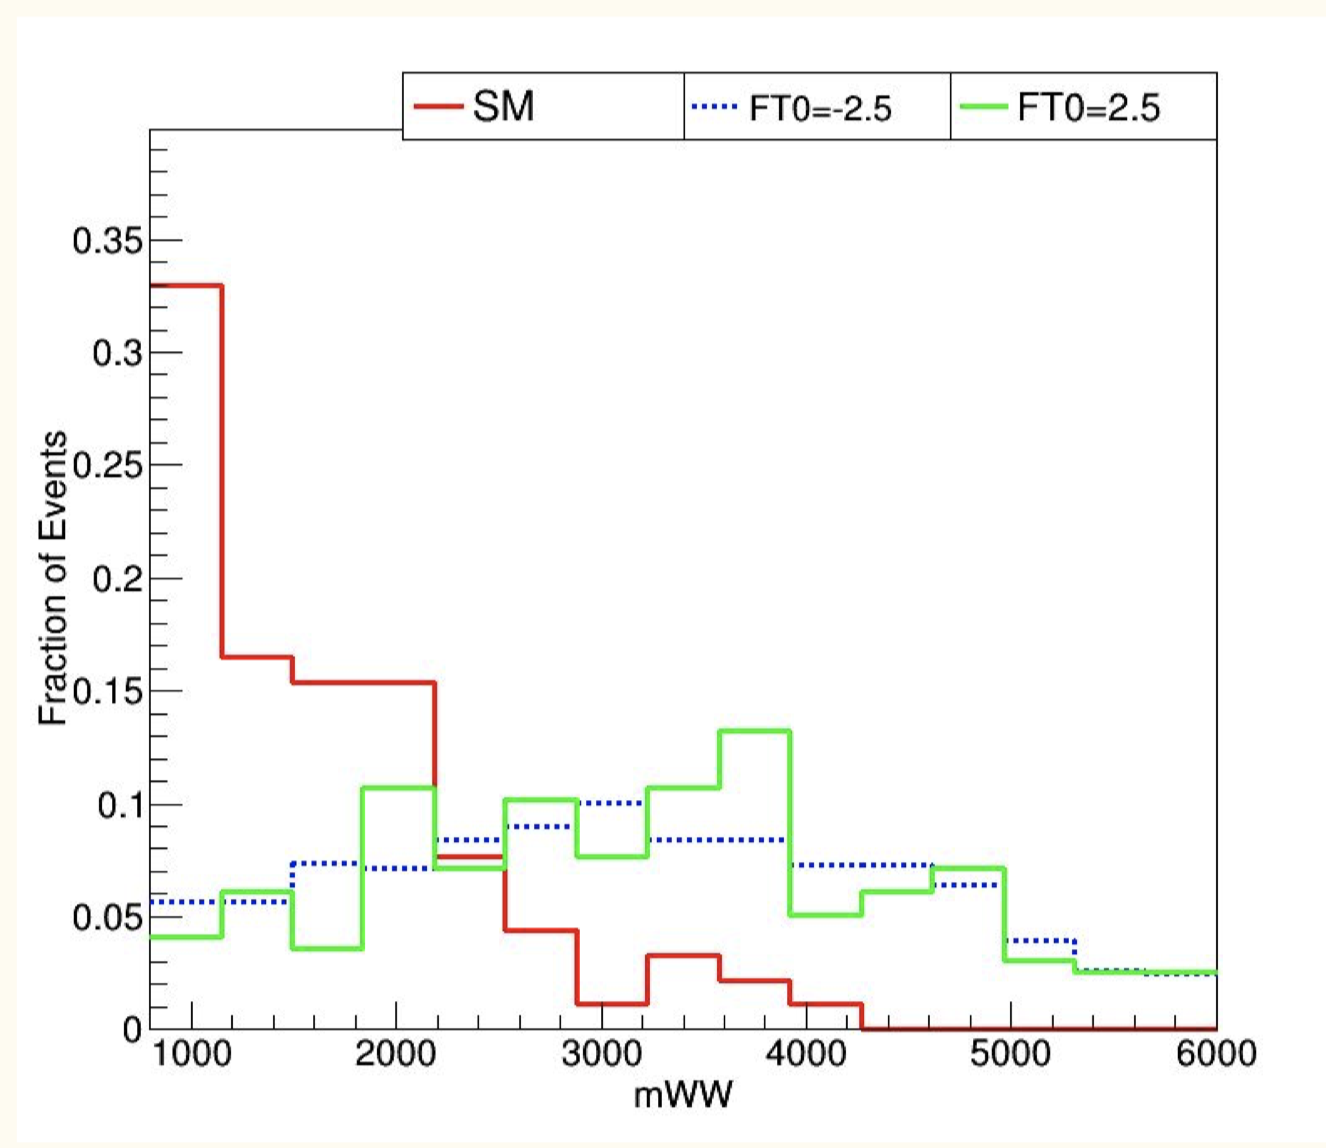
\includegraphics[width=0.90\textwidth]{Plots/GenLevelStudy/pic6.png}    \end{tabular}
    \caption{Top: W-jets distribution. Bottom: WW system invariant mass}
    \label{fig:gen3}
  \end{center}
\end{figure}
\begin{figure}[htb]
  \begin{center}
    \begin{tabular}{c}
    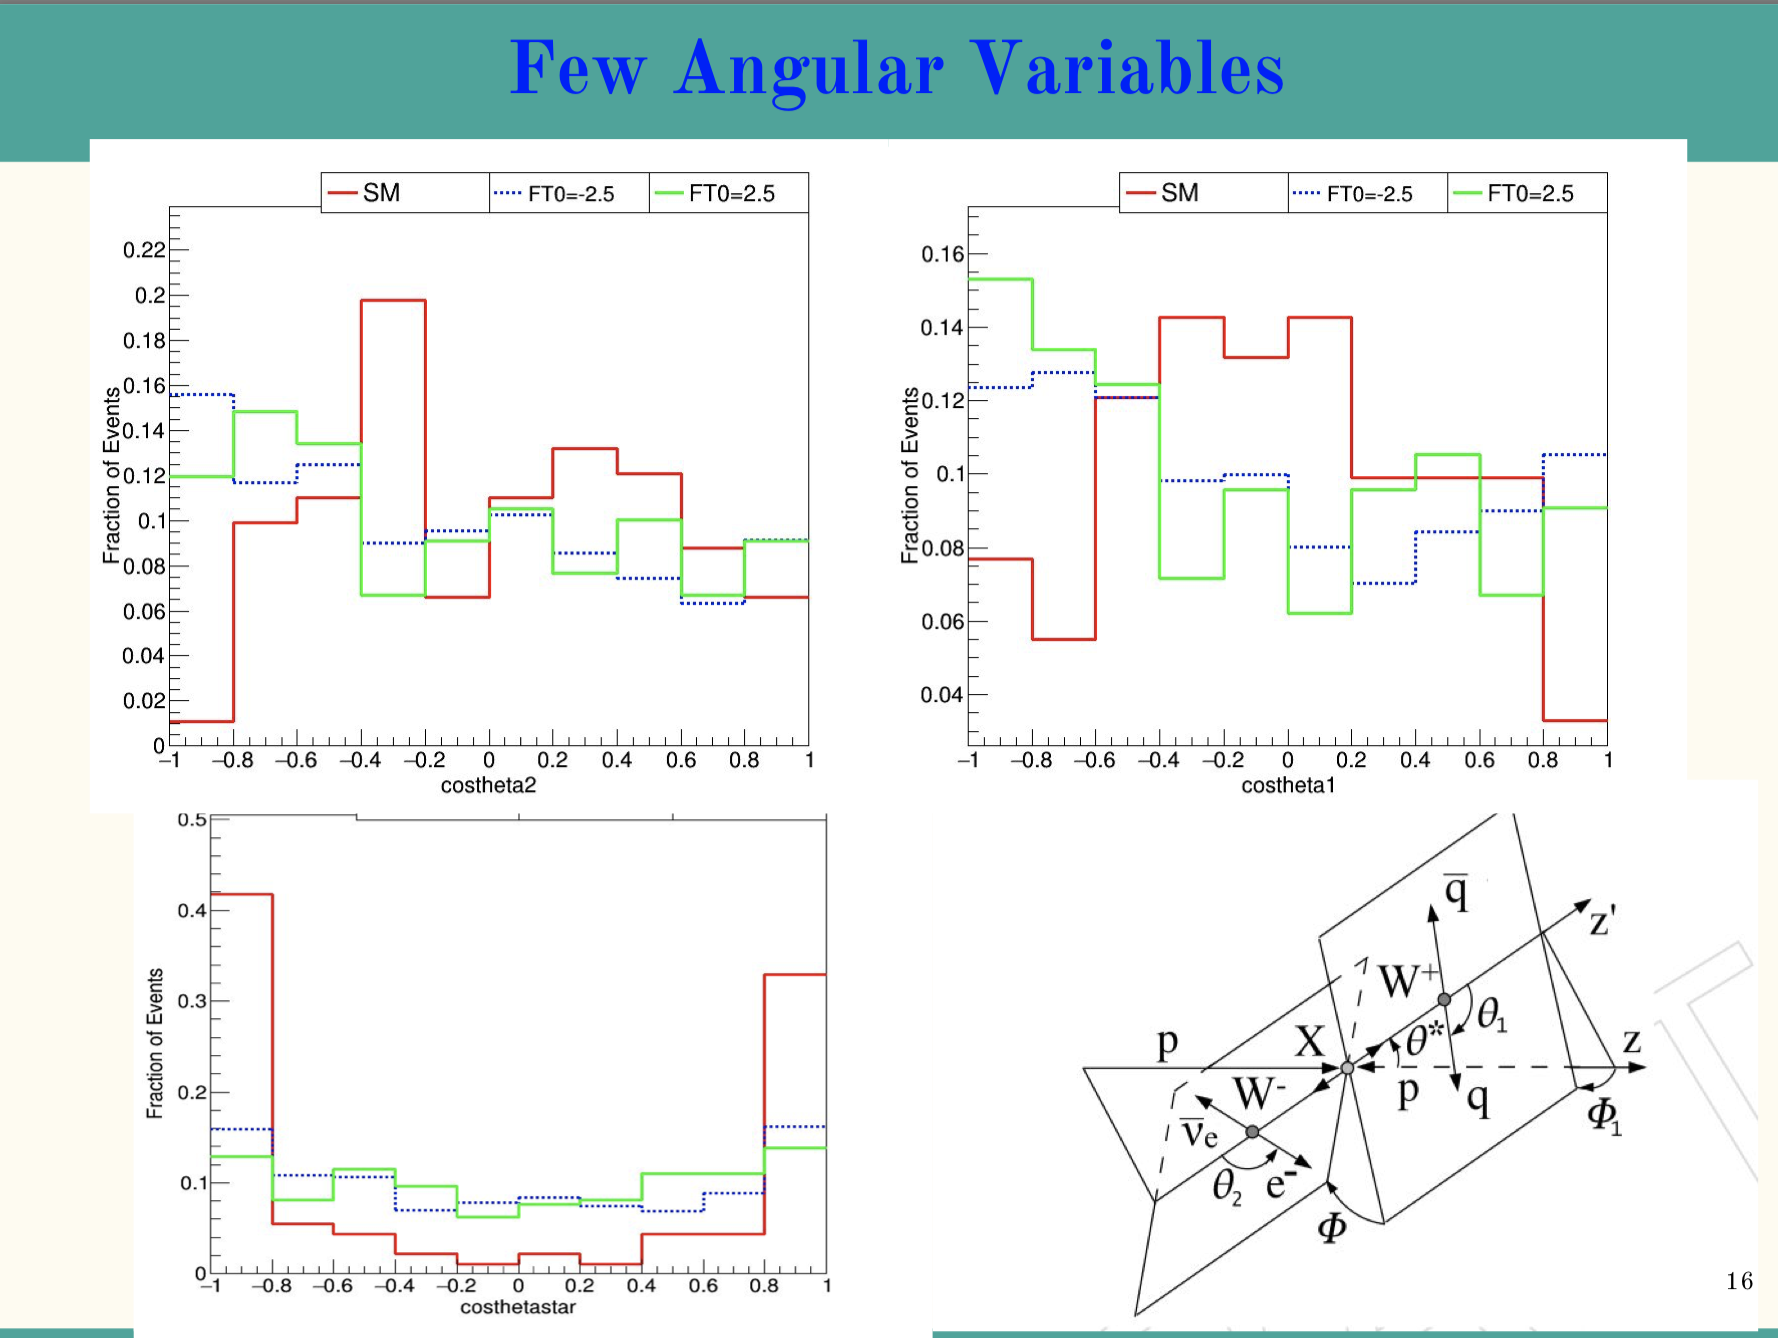
\includegraphics[width=1.00\textwidth]{Plots/GenLevelStudy/pic7.png}
    %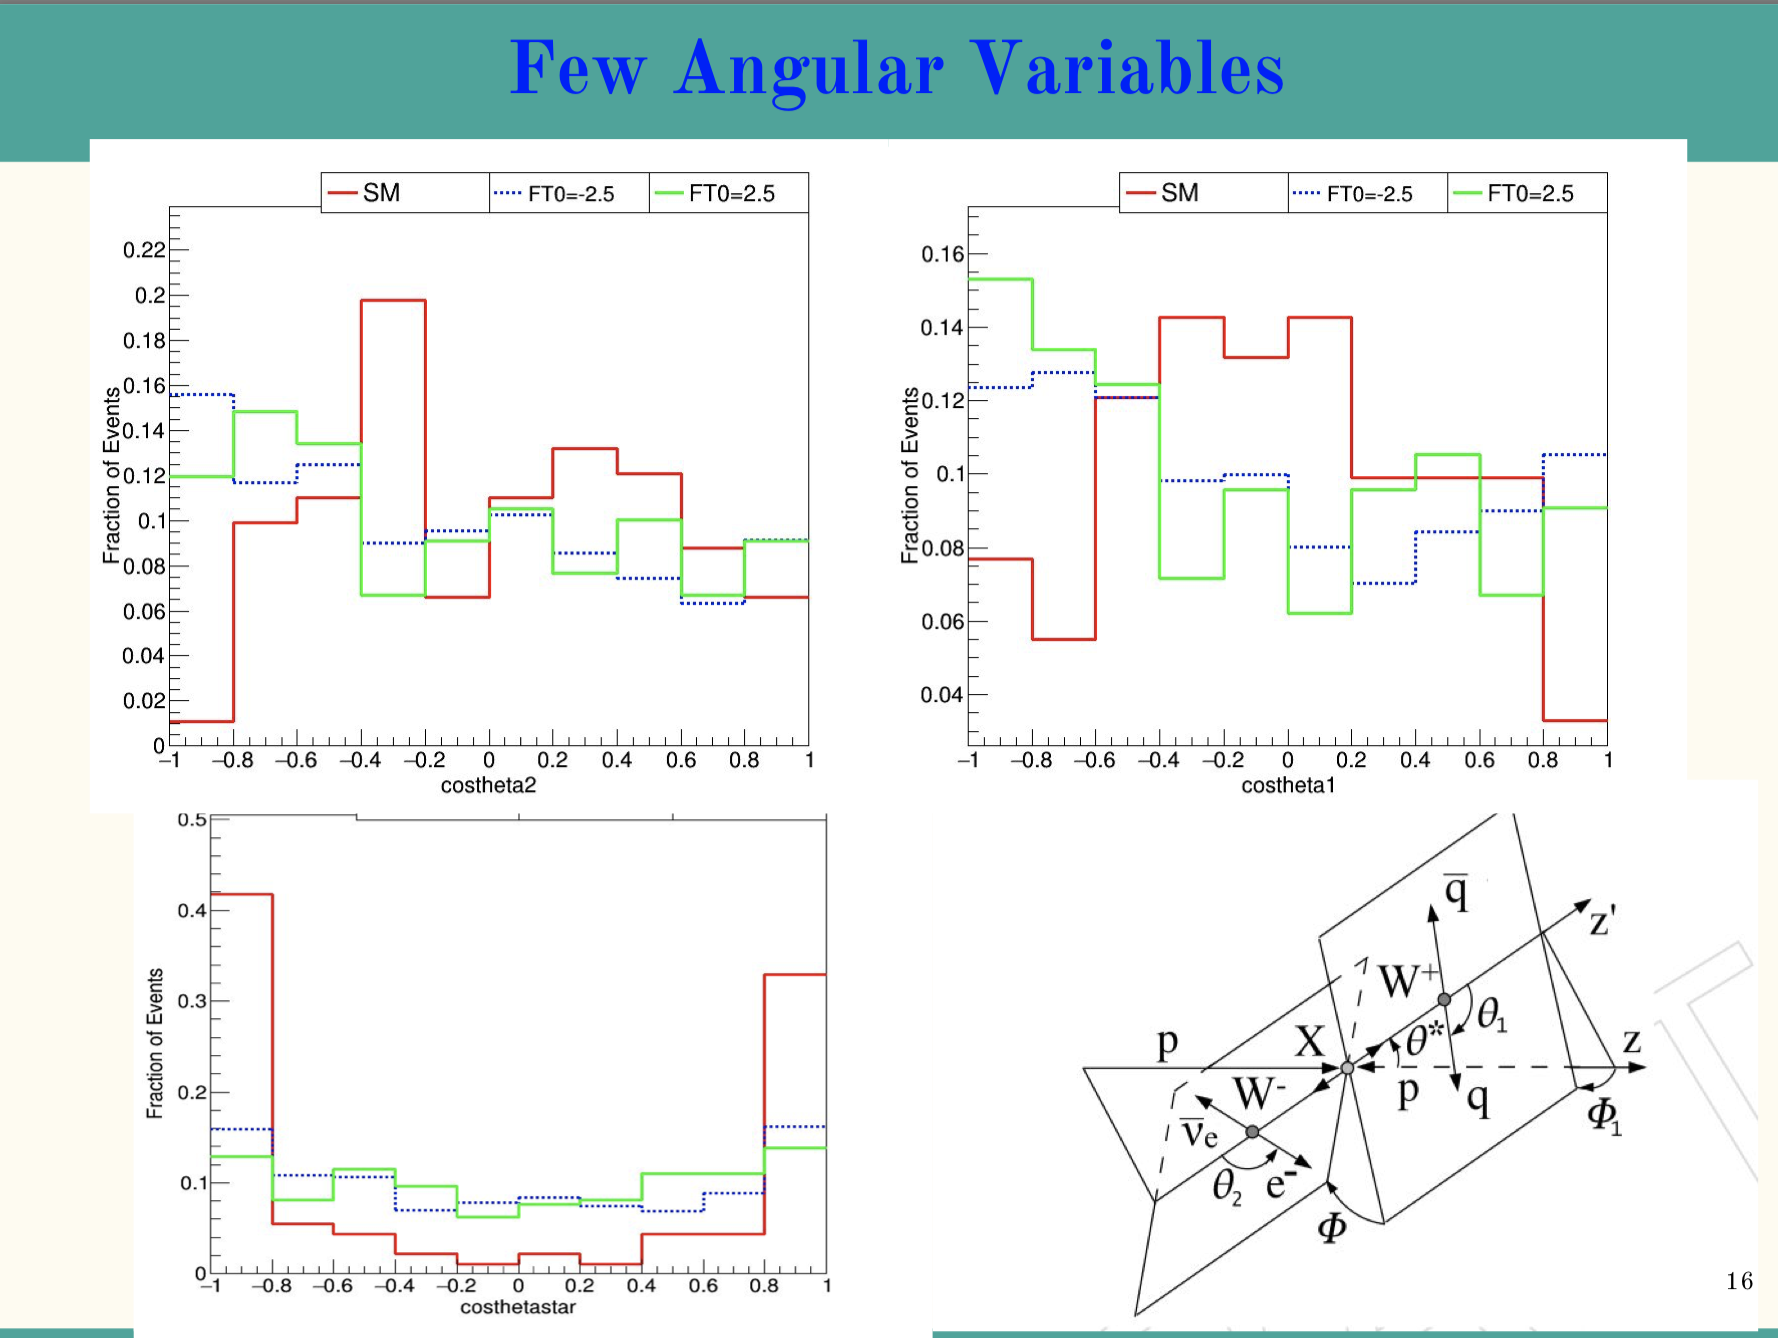
\includegraphics[width=1.00\textwidth]{Plots/GenLevelStudy/pic7.png}    
    \end{tabular}
    \caption{Angular variables}
    \label{fig:gen4}
  \end{center}
\end{figure}
%\subsubsection{Comparison of MadSpin and Decay Package of MadGraph for Polarized Sample Generation}




%\subsection{Some useful links of forum}
